\section{Inserting frames and geometries}
This section contains the description of the implementation of inserting frames and geometries. This is done trough a class called creator made specifically for creating RobWork specific objects without a XML-file description.

\subsection{General explanation of the solution}
\label{subsec:iFramesAGeomsGE}
The solution to the requirements related to insertion of frames and geometries was condensed into two parts, an interface for the information needed (GUI) and the actions needed to insert he frames with the informations gotten from the GUI. In order to simplify the process of inserting frames and geometries, with the information given, this was separated into a kind of extension to the RobWork library. The name chosen for this extension was creator since its focus was on creating and adding elements from the RobWork library.\\

Separating the problem into the GUI and creator have several benefits. First of all, it has the benefit of modularity. The creator is not dependant on a the GUI and is written in a way that allows use in other applications than this one.\\
Another reason is that it makes it easier to divide the task as long as the interface to the GUI is agreed on.

\subsection{Using the creator}
The creator follows the same namespacing technique as RobWork employ in order to make it more intuitive to use besides RobWork. However instead of using rw as the first namespace, ei (for EasyInsert) is used. This could be changed to rw in order make the blend perfect, however it was chosen not to in order to make the user aware that the creator is not part of the RobWork library.\\

In the case of frames the creator is capable of creating fixed frames and movable frames. The creator is also able to add them to a supplied WorkCell and in the case of the movable frame, give it an initial transform in the WorkCell. The fixed frame should always be supplied with a transform. 
Both functionalities returns a handle to the newly created frame which the user can user instead of being forced to search the WorkCell for the pointer after creating the frame.\\

In the case of geometries the creator is capable of adding 6 different geometries to a specified WorkCell: boxes, planes, spheres, cones, cylinders and tubes. No matter what geometry the user wishes to create, the user needs to provide the WorkCell. The user also needs to provide a pointer to the frame they wish to include geometry to. Instead of this the user can supply the name of a parent frame for a new movable frame on which the geometry is put. The user also needs to provide the necessary information in order to create the different geometries. This varies between the different geometries, a list of the different inputs need for the different geometries can be seen on figure~\ref{fig:InputsForGeoms}. It is also possible to supply the function with a transform which then represents the local transformation of the object in relation to the frame on which it has been included.\\

\begin{figure}[h]
	\centering
	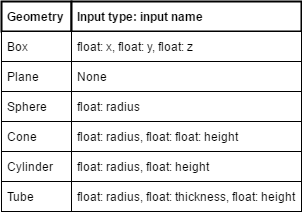
\includegraphics[scale=0.55]{Figures/InputsForGeoms.png}
	\caption{Table of geometric specific inputs for the individual geometries}
	\label{fig:InputsForGeoms}
\end{figure}

Since a lot of transformations are used in the creator it was decided also to create a function to easily create transform objects from R,P,Y and x,y,z values. The function (called getTransform3D) takes in these values and returns a Transform3D object.\\

An example of adding a sphere to a new WorkCell can be seen on figure~\ref{fig:CodeExampleAddSphere}.

\begin{figure}[h]
	\centering
	\lstset{language=C++} 
	\begin{lstlisting}[frame=single]
	// Create new wc
	WorkCell::Ptr dummy = ownedPtr(new WorkCell("wc"));
	 
	// Radius of 10 cm
	float radius = 0.1;
	
	// Displacement of 10 cm in x, y and z
	Transform3D<double> transform = getTransform3D(0.1, 0.1, 0.1, 0, 0, 0); 
	
	// Adding sphere to WorkCell
	ei::creator::addSphere( "testSphere", // Name of Sphere
							"WORLD", // Name of parent frame
							wc, // Pointer to WorkCell
							radius, // Radius of Sphere
							transform); // Transform of Sphere
	 
	\end{lstlisting}
	\caption{Code example of adding a sphere to a new WorkCell. The sphere has a radius of 10 cm and a displacement of 10 cm in x, y and z in relation to the frame on which it is set. The sphere is added to a new movable frame with the parent set to the WORLD frame.}
	\label{fig:CodeExampleAddSphere}
\end{figure}

\subsection{Implementation of the creator}
The creator was implemented with the purpose of using the most upper layers of the RobWork libraries functions to solve as much of the problem as possible. This was done since in RobWork it is possible to access lower levels of the library which makes the RobWork library way more flexible. An example of this could be when working with the frames of a WorkCell the upper layer way of doing it would be accessing the frames through the WorkCell's own functionality for getting frames, whereas the lower layer of doing it would be to access the state structure in the WorkCell and through it access the frames. The other reasoning for using upper layers is that it is usually simpler code, meaning there is less mistakes to make and the mistakes made are easier to find.\\

The implementation of the getTransform3D function is rather simple since it utilises some conversions in the RobWork library. The inputs for the function are 6 doubles representing the x, y, z displacement and the R, P, Y values representing the rotation. In order to create a Transform3D object, a vector representing the displacement and a matrix representing the rotation is needed. The displacement vector is easy to create since it is just a vector containing the values directly from the input. The rotation matrix however is more difficult to get since the input for the rotation is represented in R, P, Y values. The R, P, Y values needs to be converted to a rotation matrix. Instead of doing the calculations manually, RobWork, albeit a little hidden, can do this for us through the RPY class in the math namespace. First an RPY object is created with the values from the input. Then the member function toRotation3D from the RPY class is called returning the rotation matrix of the given R, P, Y values. The displacement vector and rotation matrix is then used to create a Transform3D object that is returned to the user. It would be possible to just implement the same functionality that the toRotation3D RPY class, eliminating the creation of an RPY object. This would increase the computation speed, but not significantly unless the function is used a lot.

\subsubsection{Implementation of creating and adding frames}
There are a total of 4 functions in the creator that are related to creating and adding frames to a WorkCell. The first 2, one for each type of frame, are functions related to creating frames. The implementation of creating frames in the creator is rather simple, since the process of creating frames in RobWork is simple in itself. The 2 functions are called createFixedFrame(...) and createMovableFrame(...). The createFixedFrame(...) function take the name of the frame and a transform as input, whereas the createMovableFrame(...) only takes the name as input. The functions simply call the constructor for the given frame with the provided parameters. The reasoning behind having these rather simple functionalities is in the context that the creator should be consistent in the functionality it embodies. Another good reason was that this was some of the first functionalities implemented for the creator. At the time the idea was that there would also be a function, atleast for the fixed frame, that took in the x, y, z and R, P, Y values instead of a transform. The function would then calculate the transform by itself and use this transform when creating the frame. This was however deemed unnecessary to implement when the getTransform3D(...) function was implemented.\\

The last 2 functions, again one for each type of frame, are functions that are capable of creating and adding a frame to a specific WorkCell. The two functions are called addFixedFrame(...) and addMovableFrame(...). Both of the functions take in a WorkCell, a name, a name of a parent frame and a transform. These functions eliminates the need for the user to understand how to create a frame and how to add the frame to the WorkCell. Even though one could say that this is rather simple process to learn, using the creator simplifies the process significantly. This comes at the cost of flexibility since the user is now locked to the implementation of the functions. However it was deemed that in many cases the functionality implemented in the creator could be used. Figure~\ref{fig:CodeExampleAddFrameDifference} showcases the standard way of creating a frame versus using the creator.

\begin{figure}[h]
	\centering
	\lstset{language=C++} 
	\begin{lstlisting}[frame=single]

	string name = "test"; // Name of frame
	string parent = "WORLD"; // Name of parent frame
	Transform3D<double> transform =  // Transform used
	ei::creator::getTransform3D(1, 1, 1, 1, 1, 1);
	WorkCell::Ptr wc; // WorkCell

	/// The standard way of adding a frame ///
	
	// Create new movable frame object and cast to frame
	MovableFrame* mframe = new rw::kinematics::MovableFrame(name);
    Frame* frame = dynamic_cast<rw::kinematics::Frame*>(mframe);
    
    // Find the parent frame in wc
    Frame* parentFrame = wc->findFrame(parent);
	
	// Test for eligible parent
	if(parentFrame != NULL) {
	
		// Add the frame to the wc
        wc->addFrame(frame, parentFrame);
		
		// Get state of wc
		State state = wc->getDefaultState();
		
		// Set transform of the movable frame in the wc
		mframe->setTransform(transform, state);
		
		// Upgrade state and update state
		state = wc->getStateStructure()->upgradeState(state); 
		wc->getStateStructure()->setDefaultState(state); 
    }
	
	
	/// Using the creator ///
	ei::creator::addMovableFrame(wc, name, parent, transform);

	\end{lstlisting}
	\caption{Code example of the standard way of adding a movable frame with a transform and the same process using the creator}
	\label{fig:CodeExampleAddFrameDifference}
\end{figure}

\subsubsection{Implementation of creating geometries}
Since in RobWork a geometry, like a box, is called an object, a way to create a object that contains the information to represent the geometry is needed. Getting inspiration from the implementation of the RWXMLLoader in RobWork, it was chosen to use the same factory approach as the loader. This means that when creating the geometry part of the object, the GeometryFactory from the loaders part of RobWork is used. When the model part of the object is created the Model3DFactory is used, again from the loaders part of RobWork. All of this is neatly put into 3 functions, addObject(...), createGeom(...) and createModel(...).\\

In order to understand process of add e.g. a box it is easiest to start from the bottom with what the factories need i order to produce the geometry and the model. From the GeometryFactory a function called load(...) is used. This function takes in a string containing the information about the geometry it needs to produce and a bool that signifies whether or not the user wishes to use cached geometries. As an example, the syntax for the string when creating a box is "\#Box dx dy dz", where dx, dy and dz are the dimensions of the box. The syntaxes for the rest of the geometries can be seen on figure~\ref{fig:SyntaxTable}.\\

\begin{figure}[h]
\centering
\begin{tabular}{|l|l|l|}
\hline
Geometry & Syntax                           & Explanation of parametres                                                                                                                    \\ \hline
Box      & "\#Box dx dy dz"                 & The dx, dy and dz are the dimensions of the box                                                                                              \\ \hline
Plane    & "\#Plane"                        & Planes need no parameters                                                                                                                    \\ \hline
Sphere   & "\#Sphere radius"                & The radius is the radius of the sphere                                                                                                       \\ \hline
Cone     & "\#Cone radius height"           & The radius is the radius of the cone and the height is the height of the cone                                                                \\ \hline
Cylinder & "\#Cylinder radius height level" & The radius is the radius of the cylinder, the height is the height of the cylinder and the level is the discretization level of the cylinder \\ \hline
Tube     & "\#Tube radius height level"     & The radius is the radius of the tube, the height is the height of the tube and the level is the discretization level of the tube             \\ \hline
\end{tabular}
\caption{Table showing the syntaxes for the different geometric primitives}
\label{fig:SyntaxTable}
\end{figure}

From the Model3DFactory a function called getModel(...) is used. This function takes in a string that either describes a geometric primitive in the same syntax as the GeometryFactory or a file name. It also take a string representing the name of the model. It is rather beneficial that the input for describing the geometric primitive is the same for both the GeometryFactory and the Model3Dfactory since it makes it simpler to implement. The function addObject(...) uses both of these function when constructing the object.\\

The addObject(...) function now needs to be interfaced to the geometries. It is also known that the addObject(...) needs to be supplied string describing the geometry. To do this a series of easy to use functions related to the geometric primitives were created. An example of one of these is the addSphere(...) which takes in the necessary information to describe a sphere (the radius) and then creates the appropriate string for the factories. It then calls the addObject(...) function with this string, and other relevant information, which creates and adds the object to the WorkCell. An example of the function flow, using addSphere(...), can be seen on figure~\ref{fig:CreatorFlow}.

\begin{figure}[h]
	\centering
	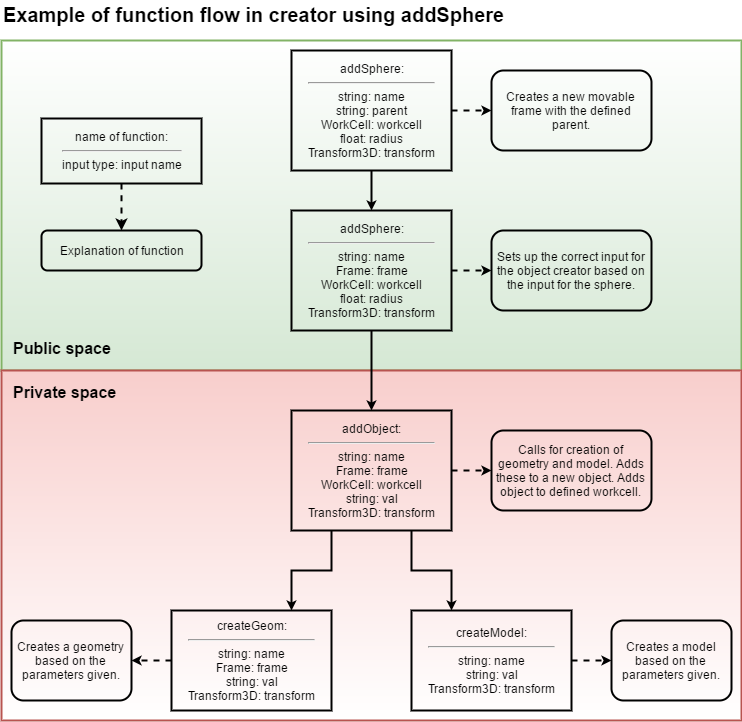
\includegraphics[scale=0.55]{Figures/CreatorFlow.png}
	\caption{Function flow of the creator using addSphere as example}
	\label{fig:CreatorFlow}
\end{figure}

\subsection{The future of the creator}
Most of the functionalities that where implemented with the purpose to fulfil the requirements of the solution. The possibilities for the creator is however almost limitless. This is mostly due to the fact that the creator is written like a library extension to the RobWork library. One of the more immediate expansions to the creator that could be made, would be to extend the geometry functions with the possibility to only create the geometry or model. This extension would make it possible to create visible objects with no collision or invisible objects with collision. Another good addition would be to create a functionality capable of loading geometries from a geometry file. This is already possible in RobWork, so it would make sense to also simplify this process in the creator.